% Options for packages loaded elsewhere
\PassOptionsToPackage{unicode}{hyperref}
\PassOptionsToPackage{hyphens}{url}
\PassOptionsToPackage{dvipsnames,svgnames,x11names}{xcolor}
%
\documentclass[
  letterpaper,
  DIV=11,
  numbers=noendperiod]{scrartcl}

\usepackage{amsmath,amssymb}
\usepackage{iftex}
\ifPDFTeX
  \usepackage[T1]{fontenc}
  \usepackage[utf8]{inputenc}
  \usepackage{textcomp} % provide euro and other symbols
\else % if luatex or xetex
  \usepackage{unicode-math}
  \defaultfontfeatures{Scale=MatchLowercase}
  \defaultfontfeatures[\rmfamily]{Ligatures=TeX,Scale=1}
\fi
\usepackage{lmodern}
\ifPDFTeX\else  
    % xetex/luatex font selection
\fi
% Use upquote if available, for straight quotes in verbatim environments
\IfFileExists{upquote.sty}{\usepackage{upquote}}{}
\IfFileExists{microtype.sty}{% use microtype if available
  \usepackage[]{microtype}
  \UseMicrotypeSet[protrusion]{basicmath} % disable protrusion for tt fonts
}{}
\makeatletter
\@ifundefined{KOMAClassName}{% if non-KOMA class
  \IfFileExists{parskip.sty}{%
    \usepackage{parskip}
  }{% else
    \setlength{\parindent}{0pt}
    \setlength{\parskip}{6pt plus 2pt minus 1pt}}
}{% if KOMA class
  \KOMAoptions{parskip=half}}
\makeatother
\usepackage{xcolor}
\setlength{\emergencystretch}{3em} % prevent overfull lines
\setcounter{secnumdepth}{5}
% Make \paragraph and \subparagraph free-standing
\ifx\paragraph\undefined\else
  \let\oldparagraph\paragraph
  \renewcommand{\paragraph}[1]{\oldparagraph{#1}\mbox{}}
\fi
\ifx\subparagraph\undefined\else
  \let\oldsubparagraph\subparagraph
  \renewcommand{\subparagraph}[1]{\oldsubparagraph{#1}\mbox{}}
\fi


\providecommand{\tightlist}{%
  \setlength{\itemsep}{0pt}\setlength{\parskip}{0pt}}\usepackage{longtable,booktabs,array}
\usepackage{calc} % for calculating minipage widths
% Correct order of tables after \paragraph or \subparagraph
\usepackage{etoolbox}
\makeatletter
\patchcmd\longtable{\par}{\if@noskipsec\mbox{}\fi\par}{}{}
\makeatother
% Allow footnotes in longtable head/foot
\IfFileExists{footnotehyper.sty}{\usepackage{footnotehyper}}{\usepackage{footnote}}
\makesavenoteenv{longtable}
\usepackage{graphicx}
\makeatletter
\def\maxwidth{\ifdim\Gin@nat@width>\linewidth\linewidth\else\Gin@nat@width\fi}
\def\maxheight{\ifdim\Gin@nat@height>\textheight\textheight\else\Gin@nat@height\fi}
\makeatother
% Scale images if necessary, so that they will not overflow the page
% margins by default, and it is still possible to overwrite the defaults
% using explicit options in \includegraphics[width, height, ...]{}
\setkeys{Gin}{width=\maxwidth,height=\maxheight,keepaspectratio}
% Set default figure placement to htbp
\makeatletter
\def\fps@figure{htbp}
\makeatother

\KOMAoption{captions}{tableheading}
\makeatletter
\@ifpackageloaded{caption}{}{\usepackage{caption}}
\AtBeginDocument{%
\ifdefined\contentsname
  \renewcommand*\contentsname{Table of contents}
\else
  \newcommand\contentsname{Table of contents}
\fi
\ifdefined\listfigurename
  \renewcommand*\listfigurename{List of Figures}
\else
  \newcommand\listfigurename{List of Figures}
\fi
\ifdefined\listtablename
  \renewcommand*\listtablename{List of Tables}
\else
  \newcommand\listtablename{List of Tables}
\fi
\ifdefined\figurename
  \renewcommand*\figurename{Figure}
\else
  \newcommand\figurename{Figure}
\fi
\ifdefined\tablename
  \renewcommand*\tablename{Table}
\else
  \newcommand\tablename{Table}
\fi
}
\@ifpackageloaded{float}{}{\usepackage{float}}
\floatstyle{ruled}
\@ifundefined{c@chapter}{\newfloat{codelisting}{h}{lop}}{\newfloat{codelisting}{h}{lop}[chapter]}
\floatname{codelisting}{Listing}
\newcommand*\listoflistings{\listof{codelisting}{List of Listings}}
\makeatother
\makeatletter
\makeatother
\makeatletter
\@ifpackageloaded{caption}{}{\usepackage{caption}}
\@ifpackageloaded{subcaption}{}{\usepackage{subcaption}}
\makeatother
\ifLuaTeX
  \usepackage{selnolig}  % disable illegal ligatures
\fi
\usepackage{bookmark}

\IfFileExists{xurl.sty}{\usepackage{xurl}}{} % add URL line breaks if available
\urlstyle{same} % disable monospaced font for URLs
\hypersetup{
  pdftitle={An Analysis of Obesity Prevelance in Scotland (2013-2016)},
  pdfauthor={Group 1},
  colorlinks=true,
  linkcolor={blue},
  filecolor={Maroon},
  citecolor={Blue},
  urlcolor={Blue},
  pdfcreator={LaTeX via pandoc}}

\title{An Analysis of Obesity Prevelance in Scotland (2013-2016)}
\author{Group 1}
\date{}

\begin{document}
\maketitle

\section{Introduction}\label{sec-intro}

Obesity occurs when an individual's energy intake from food and drink is
higher than the amount of energy needed over a period of time, and is
considered a serious public health concern. Data for this report has
been gathered from the Scottish Health Surveys from 2013-2016. The data
includes the binary variable, \texttt{Obese}, which indicates whether an
individual classes themselves as obese (Yes), or not obese (No), and the
following other lifestyle and socio-economic factors:

\begin{itemize}
\item
  \texttt{AgeGroup} - The age range of the individual (a categorical
  variable with seven different age categories).
\item
  \texttt{Sex} - The sex of an individual (a binary variable with
  categories Male or Female).
\item
  \texttt{Employment} - The individual's employment status (a
  categorical variable with seven different employment categories).
\item
  \texttt{Veg} - Indicates whether the individual consumes the
  recommended daily intake of vegetables (a binary variable with
  categories Yes or No).
\item
  \texttt{Fruit} - Indicates whether the individual consumes the
  recommended daily intake of fruit (a binary variable with categories
  Yes or No).
\item
  \texttt{Year} - The year in which the Scottish Health Survey was
  conducted (a categorical variable with categories corresponding to
  years 2013, 2014, 2015 and 2016).
\end{itemize}

The main focus of this report will be to examine the prevalence of
obesity in Scotland over the given years and to examine differences in
obesity by age, sex and the other lifestyle and socio-economic factors.

Section~\ref{sec-exploranalysis} consists of an exploratory analysis of
the obesity data and explores the potential relationship between
factors. Section~\ref{sec-formalanalysis} contains the results from
fitting a logistic regression model to the data, as well as the
assessment of the model assumptions. Concluding remarks are given in
Section~\ref{sec-conclusion}.

\section{Exploratory Analysis}\label{sec-exploranalysis}

Figure~\ref{fig-bar1} displays the relationship between variables
\texttt{Obesity} and \texttt{Year} revealing the prevalence of obesity
in Scotland over the given years of the Scottish Health Survey. From
Figure~\ref{fig-bar1}, we can see that, on average, there was not much
change in the recorded number of obese individuals in Scotland by year
from 2013 to 2016. We observe a slightly smaller count in 2016 compared
to the previous three years, but it appears that \texttt{Year} is not a
significant explanatory variable.

The proportion of no obesity has remained way above the proportion for
obesity over the given years.

\begin{figure}

\centering{

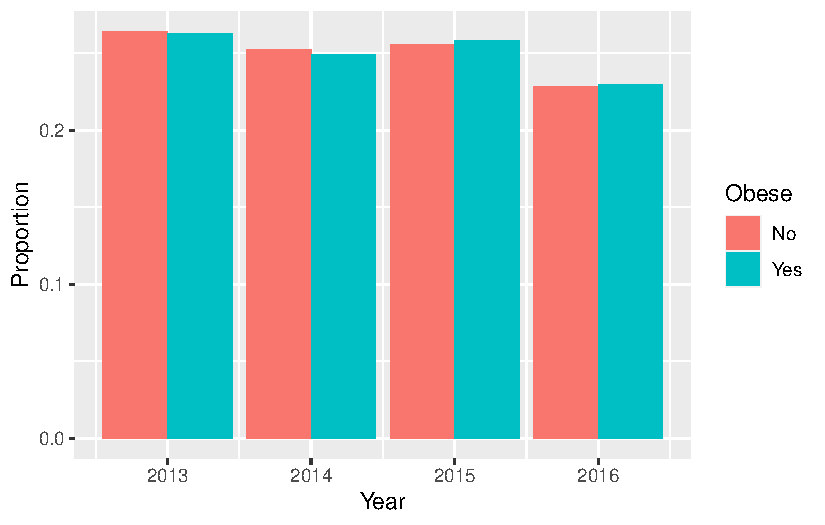
\includegraphics{Group_1_Analysis_files/figure-pdf/fig-bar1-1.pdf}

}

\caption{\label{fig-bar1}Relationship between Obesity and Year.}

\end{figure}%

In Figure~\ref{fig-bar2} we observe the relationships between
\texttt{Obesity} and \texttt{AgeGroup}, and \texttt{Obesity} and
\texttt{Sex}. It is revealed that the obesity proportion is highest in
the 55-64 age group and decreases as age decreases, as well as for an
increase in age. The lowest obesity proportion is counted in the 16-24
age group.

We can also see in Figure~\ref{fig-bar2} that obesity appears slightly
higher in females than in males.

\begin{figure}

\centering{

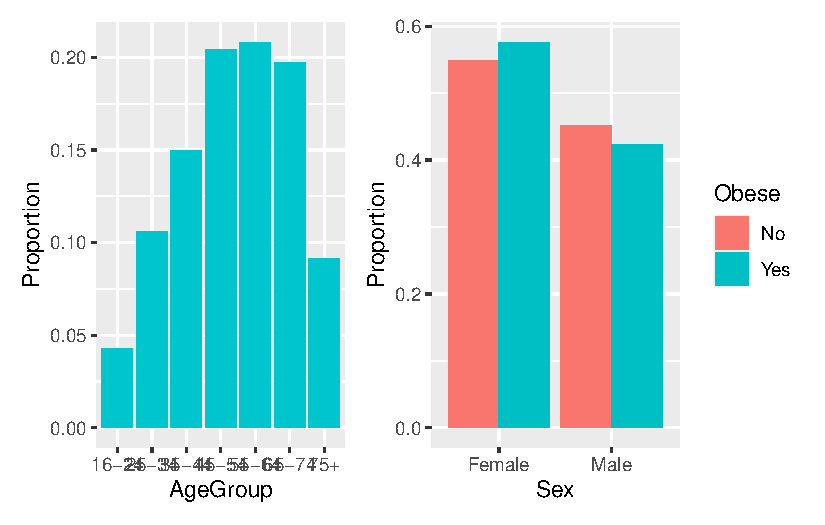
\includegraphics{Group_1_Analysis_files/figure-pdf/fig-bar2-1.pdf}

}

\caption{\label{fig-bar2}Obesity by Age Group and Sex.}

\end{figure}%

We also observe the relationship between \texttt{Obesity} and different
lifestyle factors (whether or not the individual consumes the
recommended daily intake of fruit or vegetables) in
Figure~\ref{fig-bar3}. Obesity seems to be more prevalent in those who
did consume the recommended daily intake of fruit or veg compared to
those who didn't. However, there is little to no difference between the
proportion of obese people and not obese people, so these variables
(\texttt{Fruit} in particular) seem insignificant at this stage.

\begin{figure}

\centering{

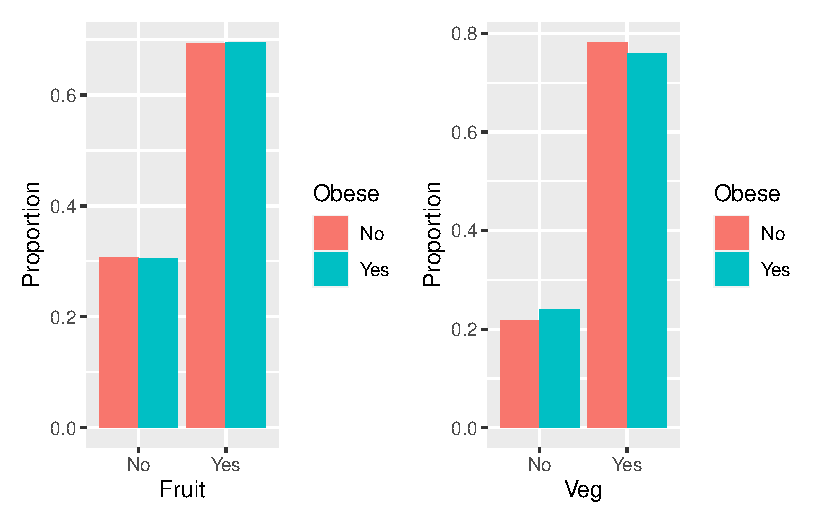
\includegraphics{Group_1_Analysis_files/figure-pdf/fig-bar3-1.pdf}

}

\caption{\label{fig-bar3}Relationship between Obesity and Lifestyle
Factors.}

\end{figure}%

The relationship between \texttt{Obesity} and \texttt{Employment} is
revealed in Figure~\ref{fig-bar4}. The obesity proportion is clearly
highest in employed individuals, followed by retirees, while the other
factors appear to have very low proportions of obesity.

\begin{figure}

\centering{

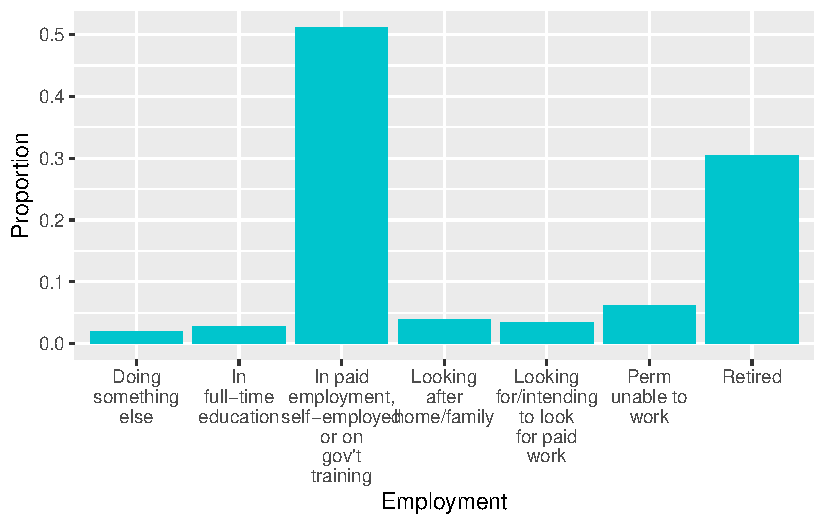
\includegraphics{Group_1_Analysis_files/figure-pdf/fig-bar4-1.pdf}

}

\caption{\label{fig-bar4}Relationship between Obesity and Socio-economic
Status.}

\end{figure}%

Finally Figure~\ref{fig-bar5} is plotted to see if there is any
relationship between \texttt{AgeGroup} and \texttt{Sex}. Initial
inspection of Figure~\ref{fig-bar5} highlights that there does seem to
be some difference between proportions of \texttt{Sex} by
\texttt{AgeGroup} between some of the age groups, so we may want to fit
the interaction between these variables in our model.

\begin{figure}

\centering{

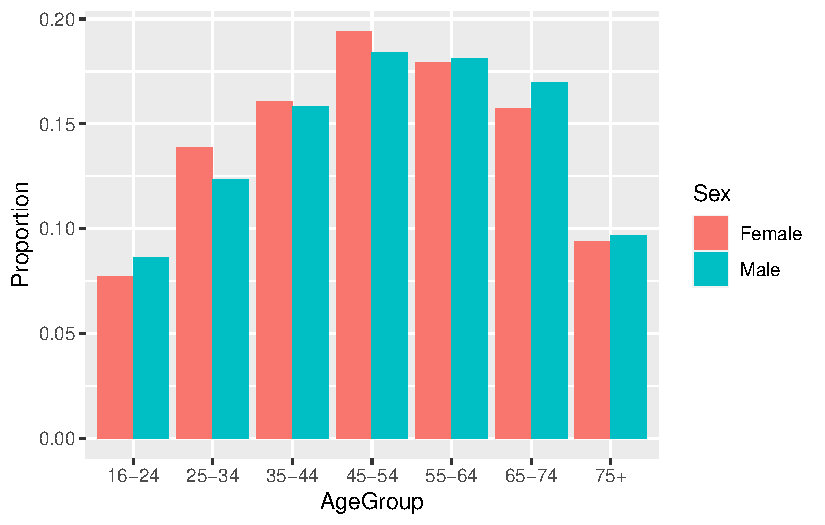
\includegraphics{Group_1_Analysis_files/figure-pdf/fig-bar5-1.pdf}

}

\caption{\label{fig-bar5}Relationship between Age and Sex.}

\end{figure}%

\section{Formal Analysis}\label{sec-formalanalysis}

To analyse the prevalence of obesity over the given years, we produce a
logistic regression model for \texttt{Obesity} by \texttt{Year}. The
large p-values shown in Figure~\ref{fig-GLMyear} match our assumptions
from Figure~\ref{fig-bar1}: we can conclude that year has no significant
effect on obesity in Scotland.

\begin{figure}

\centering{

\begin{longtable*}[]{@{}lrrrr@{}}
\toprule\noalign{}
& Estimate & Std. Error & z value &
Pr(\textgreater\textbar z\textbar) \\
\midrule\noalign{}
\endhead
\bottomrule\noalign{}
\endlastfoot
(Intercept) & -0.8330257 & 0.0358072 & -23.2642066 & 0.0000000 \\
Year2014 & -0.0056340 & 0.0512792 & -0.1098688 & 0.9125134 \\
Year2015 & 0.0162645 & 0.0508975 & 0.3195548 & 0.7493058 \\
Year2016 & 0.0111467 & 0.0524656 & 0.2124565 & 0.8317509 \\
\end{longtable*}

}

\caption{\label{fig-GLMyear}GLM with Year as explanatory variable.}

\end{figure}%

Now we go ahead and fit a model in order to analyse the relationship
between obesity and our other variables. The \texttt{Year} and
\texttt{Fruit} variables are not included in our initial fit of the
model: our exploratory analysis concluded that these variables do not
appear to impact obesity. Also, there does not appear to be any
interaction between sex and employment so we remove this interaction
from the final model. The \texttt{StepAIC} function from the
\texttt{MASS} package is then used to fit the model with the lowest AIC,
the output of which is displayed in Figure~\ref{fig-GLMfull}.

Since the baseline category for our response (\texttt{Obese}) is ``No'',
the estimates from our fitted logistic regression model are for changes
in the log-odds for individuals that answered ``Yes'' to the obesity
self evaluation compared with the log-odds of those who answered ``No''.

\begin{figure}

\centering{

\begin{longtable*}[]{@{}
  >{\raggedright\arraybackslash}p{(\columnwidth - 12\tabcolsep) * \real{0.4610}}
  >{\raggedleft\arraybackslash}p{(\columnwidth - 12\tabcolsep) * \real{0.0780}}
  >{\raggedleft\arraybackslash}p{(\columnwidth - 12\tabcolsep) * \real{0.0780}}
  >{\raggedleft\arraybackslash}p{(\columnwidth - 12\tabcolsep) * \real{0.0780}}
  >{\raggedleft\arraybackslash}p{(\columnwidth - 12\tabcolsep) * \real{0.1348}}
  >{\raggedleft\arraybackslash}p{(\columnwidth - 12\tabcolsep) * \real{0.0851}}
  >{\raggedleft\arraybackslash}p{(\columnwidth - 12\tabcolsep) * \real{0.0851}}@{}}
\toprule\noalign{}
\begin{minipage}[b]{\linewidth}\raggedright
\end{minipage} & \begin{minipage}[b]{\linewidth}\raggedleft
Estimate
\end{minipage} & \begin{minipage}[b]{\linewidth}\raggedleft
Std. Error
\end{minipage} & \begin{minipage}[b]{\linewidth}\raggedleft
z value
\end{minipage} & \begin{minipage}[b]{\linewidth}\raggedleft
Pr(\textgreater\textbar z\textbar)
\end{minipage} & \begin{minipage}[b]{\linewidth}\raggedleft
Lower.Bound
\end{minipage} & \begin{minipage}[b]{\linewidth}\raggedleft
Upper.Bound
\end{minipage} \\
\midrule\noalign{}
\endhead
\bottomrule\noalign{}
\endlastfoot
(Intercept) & -1.2235057 & 0.1738140 & -7.0391675 & 0.0000000 &
-1.5641811 & -0.8828303 \\
VegYes & -0.1654043 & 0.0444574 & -3.7205096 & 0.0001988 & -0.2525409 &
-0.0782677 \\
SexMale & -0.5692815 & 0.1690166 & -3.3681993 & 0.0007566 & -0.9005539 &
-0.2380090 \\
EmploymentIn full-time education & -0.2906684 & 0.1746231 & -1.6645479 &
0.0960030 & -0.6329297 & 0.0515928 \\
EmploymentIn paid employment, self-employed or on gov't training &
-0.0315053 & 0.1341119 & -0.2349182 & 0.8142723 & -0.2943647 &
0.2313541 \\
EmploymentLooking after home/family & 0.3753494 & 0.1652890 & 2.2708674
& 0.0231550 & 0.0513830 & 0.6993159 \\
EmploymentLooking for/intending to look for paid work & 0.2481246 &
0.1661824 & 1.4930859 & 0.1354147 & -0.0775929 & 0.5738420 \\
EmploymentPerm unable to work & 0.4425461 & 0.1550018 & 2.8551023 &
0.0043023 & 0.1387425 & 0.7463497 \\
EmploymentRetired & 0.0492760 & 0.1475305 & 0.3340053 & 0.7383756 &
-0.2398838 & 0.3384358 \\
AgeGroup25-34 & 0.3078846 & 0.1300082 & 2.3681932 & 0.0178752 &
0.0530685 & 0.5627007 \\
AgeGroup35-44 & 0.5110762 & 0.1272830 & 4.0152735 & 0.0000594 &
0.2616015 & 0.7605510 \\
AgeGroup45-54 & 0.6320838 & 0.1249245 & 5.0597261 & 0.0000004 &
0.3872318 & 0.8769359 \\
AgeGroup55-64 & 0.6181911 & 0.1281306 & 4.8246967 & 0.0000014 &
0.3670552 & 0.8693270 \\
AgeGroup65-74 & 0.7747508 & 0.1438577 & 5.3855361 & 0.0000001 &
0.4927897 & 1.0567119 \\
AgeGroup75+ & 0.5615485 & 0.1563394 & 3.5918562 & 0.0003283 & 0.2551234
& 0.8679737 \\
SexMale:AgeGroup25-34 & 0.3122112 & 0.2026095 & 1.5409504 & 0.1233289 &
-0.0849034 & 0.7093258 \\
SexMale:AgeGroup35-44 & 0.3481537 & 0.1939381 & 1.7951794 & 0.0726251 &
-0.0319650 & 0.7282725 \\
SexMale:AgeGroup45-54 & 0.4999260 & 0.1885342 & 2.6516455 & 0.0080101 &
0.1303989 & 0.8694531 \\
SexMale:AgeGroup55-64 & 0.7277964 & 0.1888479 & 3.8538772 & 0.0001163 &
0.3576547 & 1.0979382 \\
SexMale:AgeGroup65-74 & 0.5708148 & 0.1901281 & 3.0022645 & 0.0026798 &
0.1981638 & 0.9434659 \\
SexMale:AgeGroup75+ & 0.2372185 & 0.2088176 & 1.1360084 & 0.2559531 &
-0.1720639 & 0.6465009 \\
\end{longtable*}

}

\caption{\label{fig-GLMfull}Summary of regression coefficients for the
final model}

\end{figure}%

Figure~\ref{fig-GLMfull} shows each of the parameters that are included
in the final model. The selected model with the lowest AIC includes
variables \texttt{Veg}, \texttt{Sex}, \texttt{Employment},
\texttt{AgeGroup} and an interaction term between \texttt{Sex} and
\texttt{Agegroup}. The equation for the full fitted model is formally
written below:

\begin{equation*}
  \begin{aligned}
    \ln\left(\frac{p}{1-p}\right) &= -0.165\cdot\mathbb{I}_\text{Veg} -0.569\cdot\mathbb{I}_\text{Male}  -0.291\cdot\mathbb{I}_\text{Full-time Employment} \\
    &-0.032\cdot\mathbb{I}_\text{In Paid Employment/Self Employed/Govt Training} 
+0.375\cdot\mathbb{I}_\text{Looking after home/family} \\

&+ 0.248\cdot\mathbb{I}_\text{Looking for/Intending to look for work} +0.443\cdot\mathbb{I}_\text{Perm unable to work} + 0.049\cdot\mathbb{I}_\text{Retired} \\ 

&+0.308\cdot\mathbb{I}_\text{25-34} +0.511\cdot\mathbb{I}_\text{35-44} +0.632\cdot\mathbb{I}_\text{45-54} + 0.618\cdot\mathbb{I}_\text{55-64} + 0.775\cdot\mathbb{I}_\text{65-74} \\ 

&+0.562\cdot\mathbb{I}_\text{75+}+ 0.312\cdot\mathbb{I}_\text{Male and 25-34} + 0.348\cdot\mathbb{I}_\text{Male and 35-44} + 0.500\cdot\mathbb{I}_\text{Male and 45-54} \\

&+ 0.723\cdot\mathbb{I}_\text{Male and 55-64} + 0.571\cdot\mathbb{I}_\text{Male and 65-74} + 0.237\cdot\mathbb{I}_\text{Male and 75+} \\
  \end{aligned}
\end{equation*}

Where, \(\mathbb{I}\) is an indicator function and
\(p = \text{Prob}(\text{Obese})\). The equation above highlights how the
log-odds of an obese individual change by the various lifestyle and
socio-economic factors. This gives us estimates for the log-odds, and
therefore odds, for each individual in the survey.

In order to examine ranges of plausible log-odds of obesity for each of
the predictors in the fitted model equation, we can observe the 95\%
confidence interval bounds given in Figure~\ref{fig-GLMfull} . Note that
these confidence intervals also highlight significance of the
parameters, which gives the same result as the conclusions reached from
the p-values in Figure~\ref{fig-GLMfull}.

Figure~\ref{fig-GLMfull} shows the 95\% confidence intervals for each
regression parameter included in the fitted model. For example, we are
95\% confident that the log-odds of an individual being obese is, on
average, 0.078 to 0.252 lower if the individual eats vegetables.

\subsection{Assessing model
assumptions}\label{assessing-model-assumptions}

\section{Conclusion}\label{sec-conclusion}

Obesity prevalence has shown little change between 2013 and 2016.
Obesity was found to differ by sex, age, and socio-economic and
lifestyle factors. In particular, we found that obesity was less common
in those who consumed the recommended daily intake of vegetables, but
the consumption of fruit by an individual was not a significant
predictor for obesity.

We also observed an interaction between an indivual's sex and age. There
appeared to be an increase in the odds of an individual evaluating as
obese in every category compared to females in the youngest age group.
The highest average increase in the odds was observed in males aged
55-64. So we conclude that females aged 16-24 have the lowest odds of
being obese.

In terms of socio-economic factors, we can see that there was an
increase of 1.56 in the odds of evaluating as obese among those
permanently unable to work compared to those ``doing something else''.
These odds are the highest among all employment-statuses given.



\end{document}
